\documentclass[12pt]{report}
\usepackage[utf8]{inputenc}
\usepackage{titlesec}
\usepackage[slovene]{babel}
\usepackage{acro}
\usepackage{amsmath}
\usepackage{textgreek}
\usepackage{graphicx}
\usepackage{float}
\usepackage[twoside]{fancyhdr}

\RequirePackage[backend=biber,style=numeric]{biblatex}

\addbibresource{sources.bib}
\setcounter{tocdepth}{3}
\setcounter{secnumdepth}{3}

%Okrajšave

\DeclareAcronym{PZF}{
  short=PZF,
  long=pasovno zavrnitveni filter,
}
\DeclareAcronym{MM}{
  short=MM,
  long= Metamateriali,
}
\DeclareAcronym{EVP}{
  short=EVP,
  long= problem lastnih vrednosti,
}

\DeclareAcronym{OC}{
  short=OC,
  long= osnovna celica,
}

\begin{document}

% ---- Oblikovanje strani
\pagestyle{fancy}
\renewcommand{\chaptermark}[1]{\markboth{#1}{}}

\fancyhf{}
\fancyhead[RO,LE]{\leftmark}
\fancyfoot[RO, LE]{\thepage}
% ---- Konec oblikavanja strani


\begin{titlepage}
    \begin{center}
        \textbf{UNIVERZA V LJUBLJANI}
        \\Fakulteta za strojništvo

        \vspace{5cm}
        \textbf{\Huge{3D natisnjeni metamateriali za aplikacijo v dinamiki}}

        \vspace{1cm}
        Seminarska naloga pri predmetu Dinamika togih teles

        \vspace{2cm}
        \textbf{\Large{Marko Zupan}}

        \vspace{4cm}
        Mentor: asist. Tilen Košir
        \\Somentor: prof. dr. Janko Slavič, univ. dipl. inž.

        \vspace{1.5cm}
        Ljubljana, december 2022


    \end{center}
    
\end{titlepage}

\tableofcontents

\printacronyms[name=Seznam okrajšav]

\chapter{Uvod}
\section{Cilji naloge}

Cilj naloge je izdelati numerični model in delujoč metamaterial, ki bo dušil vibracije
v željenem frekvenčnem območju. Specifično smo v okrivu naloge iskali območje dušenja
znotraj intervala 0 - 1000 Hz. Proces je bil razdeljen na 3 glavne podsklope.
\\
\\
V poglavju 2 so predstavljene teoretične osnove, ki jih potrebujemo za fizikalno razumevanje
problem in razvoj matematičnega modela, ki je osnova končnega numeričnega modela. Opisana je 
teorija nihanja sistemov z večimi prostostnimi stopnjami in teorija periodičnih struktur.
V poglavju 3 je predstavljen proces konstrukcije bazne celice in izdelave numeričnega modela. 
Opisani so osnovni koraki izdelave numeričnega modela ter predstavljeni koraki konstrukcije
osnovne celice.
V poglavju 4 je predstavljen eksperimentalni del s komentarji dobljenih rezultatov in primerjavo
z numeričnem modelom. Opisane so meritve in proces 3D tiska metamateriala.

\chapter{Teoretično ozadje}

\section{Uvod v metamateriale}
\ac{MM} so na makro nivoju posebno načrtovane strukture, ki imajo zaradi posebne geometrije izboljšane
mehanske lastnosti, kakršnih ne najdemo v naravi. \ac{MM} se uprabljajo na različnih področjih,
med njimi tudi v dinamiki. Na tem področju nas zanimajo \ac{MM}, ki so sposobni tvoriti \ac{PZF}. \ac{PZF} 
predstavlja frekvenčno področje, v katerem \ac{MM} teoretično ne dopušča prostega širjenja valovanja.
Znotraj takih področij lahko zato pričakujemo močno slabljenje vibracij.
\\
\\
\ac{PZF} lahko kreiramo prek dveh različnih mehanizmov. Prvi uporablja fizikalni princip Braggovega sipanja
 (ang. Bragg Scattering). Značilnost tovrstnega principa je periodična struktura \ac{MM} iz osnovnih gradnikov,
 ki vsebujejo visoke impedančne spremembe. To povzroča sipanje valovnih dolžin, ki so primerljive karakterističi dolžini 
 osnovnega gradnika. Pri Braggovem sipanju prihaja do destruktivne interference prihajajočega in odbitega vala, kar povzroči
 delno ali popolno izničenje valov. Ta princip je primeren le za tvorbo \ac{PZF} pri višjih frekvencah, kar ne ustreza
 ciljem te naloge.
 \\
 \\
 Drugi mehanizem deluje na principu lokalnih resonanc \ac{MM}. V okviru tega mehanizma na strukturo periodično namestimo
 lokalne resonatorje. Resonančni \ac{PZF} v tem primeru ni odvisen od periodičnosti, temveč geometrijskih lastnosti resonatorja. 
 Pogoja za nastanek \ac{PZF} sta majhna medsebojna oddaljenost resonatorjem (nekaj velikostnih razredov nižje od valovnih dolžin frekvenc,
 ki bi jih radi dušili) in ne-ničelna inducirana rezultantna sila na osnovno strukturo. Prednost tovrstnega pristopa je zmožnost kreiranja
 \ac{PZF} tudi pri nižjih frekvencah, slabosta pa, da lahko izven tega področja tudi močno poslabšamo slabljenje vibracij. \cite{kosir}
 \\
V okrviru te naloge se bomo osredotičli na konstruiranje 1D \ac{MM} preko mehanizma lokalnih resonatorjev.

\section{Osnove lastnih nihanj sistemov z več prostostnimi stopnjami}
V okviru tega poglavja predpostavimo, da že poznamo enačbe opazovanega sistema z več prostostnimi stopnjami, kot je 
prikazano na enačbi (2.1), kjer upoštevamo viskozni model dušenja, čeprav bomo tega v nadaljenaju zanemarili.

\begin{equation}
  \mathbf{M} \mathbf{\ddot{q}}(t) + \mathbf{C} \mathbf{\dot{q}}(t) + \mathbf{K} \mathbf{q}(t) = \mathbf{f}(t)
\end{equation}
\\
Kjer \textbf{M} predstavlja masno matriko sistema, \textbf{C} dušilno matriko sistema, \textbf{K} togostno matriko sistema, \textbf{x}(t) in \textbf{f}(t)
pa sta vektorja generaliziranih pomikov in vzbujevalnih sil.
V nadaljevanju predpostavimo harmonski odziv, zato lahko vektor pomikov in vektor generaliziranih vzbujevalnih sil zapišemo po enačbi (2.2).

\begin{equation}
  \mathbf{q}(t)=\mathbf{q} \sin{(\omega t)} =\mathbf{q}e^{i\omega t} \\
  \mathbf{f}(t)=\mathbf{f} \sin{(\omega t)} =\mathbf{f}e^{i\omega t}
\end{equation}
\\
Kjer \textbf{q} predstavlja vektor amplitud generaliziranih pomikov, \textbf{f} pa vektor generaliziranih vzbujevalnih sil. Če enačbo (2.1) preuredimo s pomočjo enačbe (2.2) dobimo sledečo enačbo
(2.3).

\begin{equation}
  (-\omega^2 \mathbf{M} + \mathbf{K}) \mathbf{q} = \mathbf{f}
\end{equation}
\\
V okviru naše naloge nas zanimajo lastne frekvence. Te dobimo iz netrivialne rešitve enačbe (2.3), ki jo dobimo z rešitvijo enačbe (2.4).
Problem prevedemo na problem lastnih vrednosti, ki je numerično stabilnejši.

\begin{equation}
  \textrm{det} (-\omega^2 \mathbf{M} + \mathbf{K})=0  
\end{equation}

\section{Metoda končnih elementov}
Metoda končnih elementov je aproksimativna metoda za reševanje matematičnih modelov in je najbolj razširjena med vsemi aproksimativnimi metodami.
Za naš primer bi lahko uporabili tudi metodo končnih elementov ali metodo robnih elementov, vendar je zaradi narave problema metoda končnih elementov najprimernejša.
S pomočjo te metode bomo pridobili globalno masno in togostno matriko \textbf{M} in \textbf{K}. 
\\
Osnovnih togostnih (2.5) in masnih (2.6) matrik za nosilec s štirimi prostostnimi stopnjami tu ne bomo izpeljevali, vendar jih pridobimo iz vira \cite{ville}.

\begin{equation}
  \mathbf{M} = \frac{\rho A l}{420} 
  \begin{bmatrix}
    156 & 22l & 54 & -13l \\
    22l & 4l^2 & 13l & -3l^2 \\
    54 & 13l & 156 & -22l \\
    -13l & -3l^2 & -22l & 4l^2
  \end{bmatrix}
\end{equation}
\begin{equation}
  \mathbf{K} = \frac{EI}{l^3} 
  \begin{bmatrix}
    12 & 6l & -12 & 6l \\
    6l & 4l^2 & -6l & 2l^2 \\
    -12 & -6l & 12 & -6l \\
    6l & 2l^2 & -6l & 4l^2
  \end{bmatrix}
\end{equation}
\\
Kjer je $\rho$ gostota, A površina preseka, l dolžina elementa, E elastični modul materiala in I vztrajnostni moment prereza.

\section{Osnove neskončnih periodičnih struktur}
Metamateriali so zaradi njihove narave navadno periodične stukture, kjer se v intervalih ponavlja osnovna celica.
Obravnavo problema si lahko olajšamo, kadar imamo neskončno periodično strukturo, saj takrat s pomočjo Bloch-Floquetovega teorema lahko 
preučujemo le odziv ene osnovne celice in tega generaliziramo na celotno strukturo.

\subsection{Bloch-Floquetov teorem}
V okviru te točke bomo predstavili osnove Bloch-Floquetovega teorema, ki ga potrebujemo za obravnavo našega problema.
Teorem nam pove, na kakšen način smemo obravnavati osnovno celico, da s tem popišemo celotno neskončno periodično strukturo \ac{MM}. \\
Omejimo se na 1D translatorno periodično strukturo z dolžino osnovne celice L. Za takšno periodično strukturo definiramo referenčni vektor $\mathbf{r}_U$, 
ki definira referenčno točko U, in referečno vektor $\mathbf{r}_P$, ki definira poljubno točko P na periodični strukturi. \cite{vanbelle, kosir}
\\Povezava je prikazana na sliki 2.1 in v enačbi (2.7).

\begin{figure}[H]
  \centering
  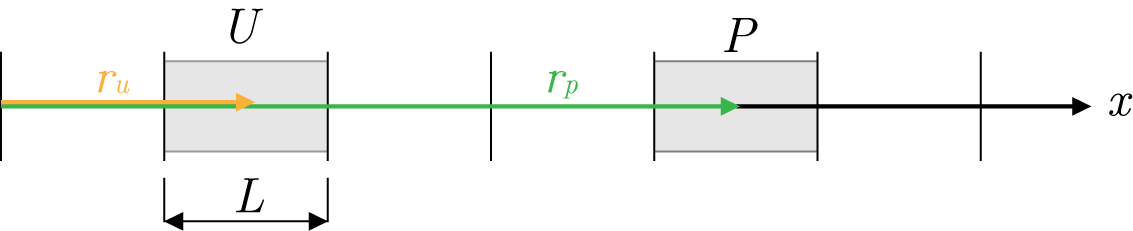
\includegraphics{Images/bloch.png}
  \caption{Prikaz 1D periodične strukture in njene bazne celice}
\end{figure}
\begin{equation}
  \mathbf{r}_P = \mathbf{r}_U + nL
\end{equation}
Kjer L ponazarja dolžino bazne celice, n pa celo število, ki pove število bazih celic med točkama U in P. Ponovno predpostavimo harmonsko
nihanje in tako lahko enačbo preuredimo kot:
\begin{equation}
  \mathbf{q}(r, k, t)  = \widetilde{\mathbf{q}}(r, k)e^{ik r}e^{i\omega t}
\end{equation}
Kjer r predstavlja pozicijo na x poltraku, $\omega$ frekvenco valovanja, k valovno število v smeri širjenja valovanja i pa kompleksno število. Na podlagi odziva referenčne celice
v točki U lahko napovemo odziv v katerikoli točki. Prav tako definiramo še kompleksno število širjenja valovanja $\mu$, ki nam fizikalno predstavlja fazni zamik. Preoblikovano enačbo zapišemo
kot:
\begin{equation}
  \mathbf{q}(r_P, \mu, t)  = \mathbf{q_{ref}}(r_U, \mu,t)e^{i\mu n}
\end{equation} 
Preko odziva osnovne celice lahko torej ob predpostavki neskončne periodične strukture modeliramo in napovemo odziv po celotni
periodični strukturi.

\subsection{Izračun disperzijskih krivulj}
Osnova analize širjenja valovanja znotraj osnovne strukture \ac{MM} je izračun disperzijskih krivulj. S konstrukcijo reprezentativne
osnovne celice in uporabo Bloch-Floquetovega teorema pridobimo disperzijski \ac{EVP} za frekvenco $\omega$ in valovni vektor $\mu$. \cite{vanbelle}

\subsubsection{Brillouinove cone}
Da lahko iz ravnin preidemo v krivulje, izkoriščamo periodičnost in simetrijo. Ker analiziramo periodično strukturo lahko določimo periodo 2$\pi$ za Re($\mu$) v recipročnem prostoru.
Problem razdelimo v tako imenovane Brillouinove cone. \cite{vanbelle}
\\Brillouinova cona je definirana kot Wigner-Seitzova celica v recipročnem prostoru. Najmanjši prostor, ki ga definira Wigner-Seitzova celica imenujemo prva Brillouinova cona.\cite{abhipod} Prva Brillouinova cona
je najmanjši osnovni gradnik, na podlagi katerega lahko popišemo celotno periodično strukturo. Če upoštevamo še simetrijo osnovne celice je možno slednjo cono še dodatno reducirati na nereducirno Brillouinovo cono. Ta predstavlja najmanjši prostor,
ki ga je potrebno obrvnavati, da popišemo celotni odziv osnovne celice in posledično celotnega \ac{MM}. \cite{kosir}
\\
\\
V sklopu te naloge bomo obravnavali 1D strukturo, zato se problem močno poenostavi. V ravninskem primeru bazni vektor celice \textbf{d} in bazni vektor recipročne celice \textbf{t} sovpadata s koordinatno osjo x. Poznamo tudi periodičnost, ki je enaka 2$\pi$. 
Celico transformiramo na dimenzije $[-\pi, \pi]$ s koordinatnim sistemom $\mu$, kot je prikazano na sliki (2.3).

\begin{figure}[H]
  \centering
  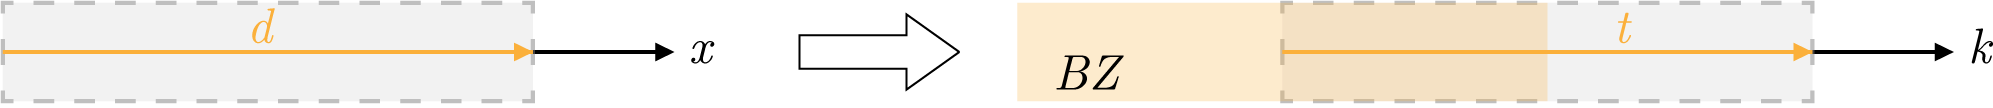
\includegraphics[scale=0.8]{Images/osnovna_celica.png}
  \caption{Bazne celice, njena recipročna celica v prostoru in Brillouinova cona (BZ)}
\end{figure}
\begin{figure}[H]
  \centering
  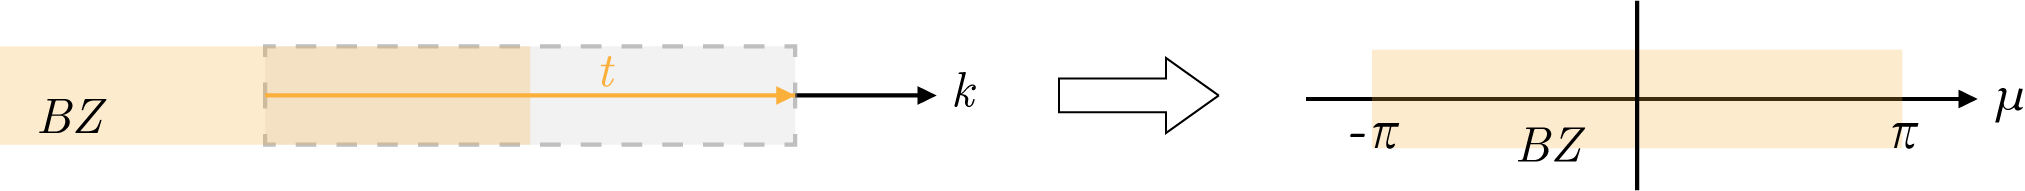
\includegraphics[scale=0.8]{Images/transformacija.png}
  \caption{Transformacija Brillouinove cone iz valovnega (k) v valovni ($\mu$) prostor}
\end{figure}

\subsubsection{Modeliranje osnovne celice}
V poglavju 2.2 smo izpeljali vodilno enačbo problema (2.3), kjer smo dobili dinamsko matriko:
\begin{equation}
  \mathbf{\hat{D}}(\omega)= -{\omega}^2 \mathbf{M}+K
\end{equation}
Sledeča dinamska matrika zaenkrat še ne vključuje nobenih robnih pogojev. V nadaljevanju bomo z uporabo Blochovega teorema za našo
dinamsko matriko določili periodične robne pogoje. Končna celica bo v numeričnem modelu imela več kot le dve vozlišči, zato v naslednjem koraku vektor pomikov $\mathbf{\hat{x}}$
razdelimo na pomike v levem vozlišču $\mathbf{q}_L$, pomike v sredini celice $\mathbf{q}_I$ in pomike v skrajnem desnem vozlišču $\mathbf{q}_R$. Vektor generaliziranih vozliščnih pomikov $\mathbf{q}$
je tako enak:
\begin{equation}
  \mathbf{q}=
    \begin{Bmatrix}
      \mathbf{q}_L \\
      \mathbf{q}_I \\
      \mathbf{q}_R
    \end{Bmatrix}
\end{equation}
Uporabimo enačbo (2.9) iz Bloch-Floquetovega teorema, ki povezuje skrajna vozlišča. Tako lahko zapišemo:
\begin{equation}
  \mathbf{q}_R = \mathbf{q}_L e^{i\mu}
\end{equation}
Desno vozlišče lahko izrazimo z levim, torej se lahko znebimo ene neznanke z uporabo desne reducirne matrike $\mathbf{\Lambda_R}$:
\begin{equation}
  \mathbf{q}=\mathbf{\Lambda_R q_{red}}; \quad 
  \mathbf{q_{red}} = \begin{Bmatrix}
    \mathbf{q}_L \\
    \mathbf{q}_I
  \end{Bmatrix}; \quad
  \mathbf{\Lambda_R} = \begin{bmatrix}
    \mathbf{I} & \mathbf{0} \\
    \mathbf{I}e^{i\mu} & \mathbf{0} \\
    \mathbf{0} & \mathbf{I}
  \end{bmatrix}
\end{equation}
Kjer \textbf{I} predstavlja identično matriko \textbf{0} pa matriko ničel.\\
Podobno naredimo tudi za vektor generalizirnih vozliščnih sil, kjer upoštevamo konsistentnost notranjih veličin:
\begin{equation}
  \mathbf{f}_R = -\mathbf{f}_L e^{i\mu}
\end{equation}
Desno vozlišče lahko izrazimo z levim, torej se lahko znebimo ene neznanke z uporabo leve reducirne matrike $\mathbf{\Lambda_L}$:
\begin{equation}
  \mathbf{f}=\mathbf{\Lambda_L f_{red}}; \quad 
  \mathbf{f_{red}} = \begin{Bmatrix}
    \mathbf{f}_L \\
    \mathbf{f}_I
  \end{Bmatrix}; \quad
  \mathbf{\Lambda_L} = \begin{bmatrix}
    \mathbf{I} & \mathbf{I}e^{-i\mu} & \mathbf{0} \\
    \mathbf{0} & \mathbf{0} & \mathbf{I}
  \end{bmatrix}
\end{equation}
Kjer \textbf{I} predstavlja identično matriko \textbf{0} pa matriko ničel.\\
Sledeče temu postopku lahko dobimo kondenzirano dinamsko matriko $\mathbf{D}(\omega)$ \cite{kosir}. 
\\
\\
V nadaljevanju vpeljemo še reducirana vektorja generaliziranih pomikov in vozliščnih sil ter pripadajoči reducirni matriki:
\begin{equation*}
  \begin{aligned}
    \mathbf{D}(\omega)\mathbf{q}=\mathbf{f} \\
    \mathbf{D}(\omega)\mathbf{\Lambda_R q_{red}} = \mathbf{f} \\
    \mathbf{\Lambda_L} \mathbf{D}(\omega)\mathbf{\Lambda_R q_{red}} = \mathbf{\Lambda_L} \mathbf{f}
    \mathbf{\Lambda_L} \mathbf{D}(\omega)\mathbf{\Lambda_R q_{red}} = \mathbf{f_{red}}
  \end{aligned}
\end{equation*}
Zanimala nas bodo le lastna nihanja bazne celice, zato v nadaljevanju predpostavimo, da velja $\mathbf{f_{red}}=0$
Končna enačba je torej:
\begin{equation}
  \mathbf{\Lambda_L} \mathbf{D}(\omega)\mathbf{\Lambda_R q_{red}} = \mathbf{\widetilde{D}}(\omega, \mu) \mathbf{q_{red}} = 0
\end{equation}
V enačbi (2.16) imamo zajete tudi periodične robne pogoje strukture. Kot omenjeno v poglavju 2.2 sledi reševanje problema z uporabo problema
lastnih vrednosti.

\section{Izračun periodičnih struktur}
V tem poglavju bomo spoznali dva pristopa, ki jih uporabljamo za določitev \ac{PZF} za naš \ac{MM}. Rezultat obeh pristopov so disperzijske krivulje, ki popisujejo odvisnost lastne frekvence od valovnega števila 
za širjenje valovanja po neskončni periodični strukturi \ac{MM}. Metodi, ki sta opredeljeni v naslednjih podpoglavjih sta inverzni pristop, ki ga bomo uporabili za naš \ac{MM} in direktni pristop.

\subsection{Inverzni pristop}
Inverzni oz. $\omega(\mu)$ pristop privzame realni valovni vektor $\mu$, torej privzamemo proso širjenje valovanja in rešimo problem lastnih vrednosti za frekvence $\omega = \omega_{re} + i\omega_{im}$. Tak pristop ponavadi 
uporabljamo za nedušene sisteme. \cite{vanbelle} \\
Valovni vektor $\mu$ izberemo glede na Brillouinove cone, določene v poglavju 2.4.2.1. To območje diskretiziramo in rešimo \ac{EVP} dinamske matrike $\mathbf{\widetilde{D}}(\omega, \mu)$ za posamezne valovne vektorje $\mu$.
Kadar pristop uporabljamo za določanje \ac{PZF} nedušenih struktur, pričakujemo tudi realne $\omega$. \cite{kosir}

\subsection{Direktni pristop}
Direktni oz. $\mu(\omega)$ pristop pa privzame realne $\omega$, torej privzamemo časovno harmonsko širejenje valovanja. Rezultat \ac{EVP} dinamske matrike je krivulja odvisnosti valovnega vektorja $\mu$o
od $\omega$. Izračunamo valovne vektorje pri različnih $\omega$. Rezultat so valovni vektorji $\mu = \mu_{re} + i\mu_{im}$, ki so lahko realni, imaginarni ali kompleksni. Realni del predstavlja relativno spremembo amplitude, imaaginarni del pa
spremembo faze. \cite{vanbelle, kosir} Kadar je $\mu$ odvisen od večih dimenzij (2D ali 3D problem), moramo vpeljati dodatno spremenljivko, ki jo v izračunih privzamemo.
\\
\\
V našem primeru direktnega pristopa ne bomo uporabili, vendar bomo preračun izvedli le z inverznim pristopom.

\chapter{Zasnova in preračun metamateriala}
V tem poglavju je najprej predstavljena zasnovana \ac{OC} \ac{MM}. Sledi predstavitev izdelave programa za numerično simulacijo odziva \ac{MM} in izris disperzijskih krivulj po direktni
metodi.

\section{Zasnova oblike metamateriala}
Cilj zasnove je bila konstrukcija \ac{OC} \ac{MM}, ki omogoča 1D periodičnost. Zaradi lažjega prilagajanja tekom preizkusov je \ac{OC} zasnovana parametrično, kar omogoča hitre popravke
tako na nivoju CAD modela, kot tudi numeričnega izračuna. Po veliko iteracijah smo se odločili za obliko \ac{OC}, ki je prikazana na sliki (3.1). Zaradi parametričnosti lahko hitro spreminjamo 1. lastno frekvenco preko 
spreminjanja mase in togosti vzmeti resonatorja. Resonator se nahaja znotraj osnove strukture, saj tako ob nihanju strukture ne povzroča torzijskih obremenitev, prav tako pa se s tem
ognemo gibanju resonatorja v drugih smereh razen navzgor in navzdol.
\begin{figure}[H]
  \centering
  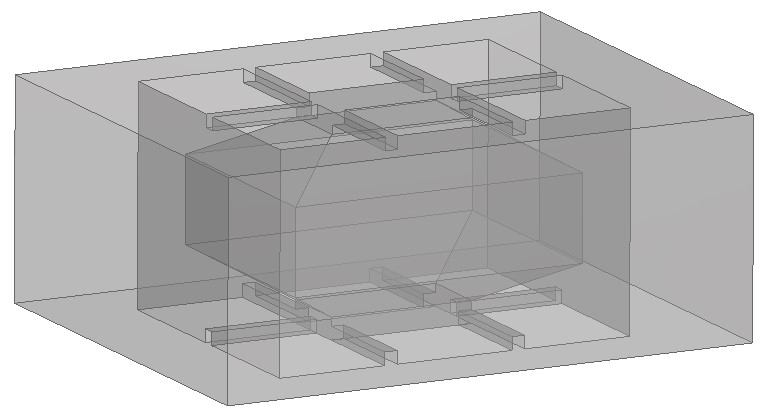
\includegraphics[scale=0.6]{Images/BaseCell_v4.JPG}
  \caption{Končni koncept \ac{OC} \ac{MM}}
\end{figure}
\noindent Pri zasnovi so bile že upoštevane tudi omejitve izdelave \ac{OC} s pomočjo FFF tehnike 3D tiska. Načrtovane vzmeti na omogočajo visoko uspešnost dobrega tiska
na dnu strukture in se zanašajo na pravilno izbrane parametre tiska pri zgornjih vzmeteh. Slednje namreč uporabljajo posebno tehniko 3D tiska imenovano ``mostiščenje'' (ang. bridging). Takrat tiskalnik nanaša material čez
večje vrzeli brez podpore. Na sliki (3.2) so prikazane končne mere \ac{OC}, ki smo jih prilagajali dokler lastna frekvenca strukture ni bila med 0 in 1000 Hz.
\\
Dvojne vzmeti na straneh so načrtovane zaradi preprečevanja nihanja notranje mase okoli z osi. Pri debelinah vzmeti smo omejeni z zmožnostjo izdelave s tehnologijo 3D tiska --- če bi
vzmeti naredili preozke ali pretanke bi prehitro prišlo do njihove porušitve.
\begin{figure}[H]
  \centering
  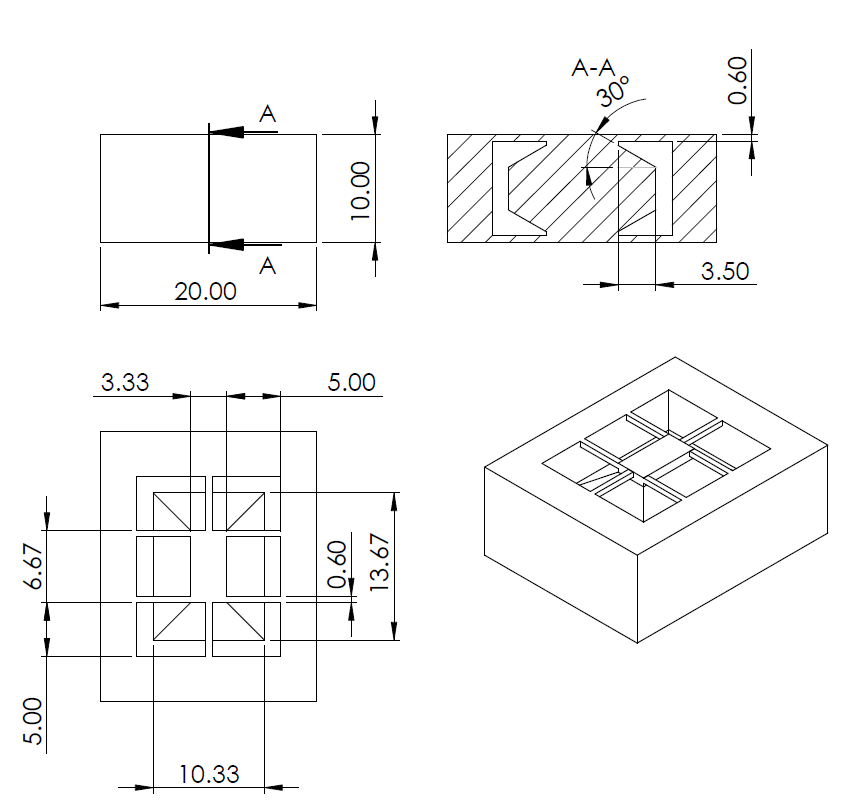
\includegraphics[scale=0.8]{Images/drawing.png}
  \caption{Dimenzije \ac{OC} \ac{MM}}
\end{figure}

\printbibliography[title={Viri}]
\end{document}